% SC3000 --- Chapter 2: Uninformed Search (0->100 ground-up)
\chapter{Uninformed Search: Breadth, Depth and Cost}
\label{ch:uninformed}

\begin{quote}
\emph{``Search is where intelligence begins.''} --- An agent that can imagine futures, try them mentally, and pick the best trip has already shown intelligence. This chapter builds \emph{blind} search from zero: no heuristic, just the map and a frontier of possibilities.
\end{quote}

\noindent\fbox{\parbox{\dimexpr\linewidth-2\fboxsep-2\fboxrule}{%
\textbf{From zero: we build here, no prior AI needed.} We define state, action, and search tree from scratch---with pictures before formulas. No heuristic or graph theory assumed. Later chapters (informed search, CSPs) reuse what is built here.}}
\vspace{0.4em}

\section*{Learning Outcomes}
After this chapter you will be able to:
\begin{enumerate}[label=(L\arabic*)]
    \item formalise any problem as a \emph{search problem} $(S,A,T,s_0,G,c)$;
    \item distinguish tree search vs.\ graph search and explain the explored set;
    \item describe the \emph{frontier} (open list) and how its discipline defines BFS, DFS, UCS, IDS;
    \item analyse completeness, optimality, time and space of each blind strategy;
    \item implement BFS and DFS/IDS and choose the right blind algorithm for a task.
\end{enumerate}

% ============================================================
\section{What Is Search? Problem Formulation}
\label{sec:search-formulation}
\emph{Intuition first.} Imagine you are lost in a subway maze with a paper map. You mark your current station, list every train you could take, and keep a \emph{to-try} list of stations you have seen but not yet explored. Search is exactly this mental simulation.

\begin{definition}[Search problem]
A search problem is a tuple $(S,A,\text{Succ},s_0,G,c)$ where $S$ is the set of \emph{states}, $A$ the set of \emph{actions}, $\text{Succ}(s)\subseteq S$ the successors of $s$, $s_0\in S$ the \emph{initial state}, $G\subseteq S$ the \emph{goal test} (often a predicate $\text{Goal}(s)$), and $c(s,a,s')\ge 0$ the step cost.
\end{definition}
A \emph{solution} is a path $s_0\to s_1\to\cdots\to s_k$ with $s_k\in G$; its cost is $\sum_{i}c(s_i,a_i,s_{i+1})$. An \emph{optimal} solution has minimum cost. The \emph{state space} is the directed graph $(S,E)$ with $E=\{(s,s'):s'\in\text{Succ}(s)\}$---distinct from the \emph{search tree} we grow while exploring.

\begin{example}[Romania road trip (Russell--Norvig)]
$S$ = cities, $s_0=$ Arad, $G=\{\text{Bucharest}\}$, $\text{Succ}(\text{Arad})=\{\text{Sibiu},\text{Timisoara},\text{Zerind}\}$, $c$ = road distance. Finding a route Arad $\to$ Bucharest is a shortest-path search problem.
\end{example}

The agent needs a \emph{node} data structure: $\langle s,\text{parent},\text{action},g\rangle$ where $g$ is path cost from $s_0$ to $s$. Expanding a node generates its successors. The set of generated-but-unexpanded nodes is the \emph{frontier} (or open list)---the boundary between explored and unseen. Which node we pick from the frontier \emph{is} the search strategy.

% ============================================================
\section{Tree Search vs.\ Graph Search and the Frontier}
\label{sec:tree-graph-frontier}
In \emph{tree search} we never remember where we have been: the same state can be generated along many paths (imagine revisiting Arad via two routes). In \emph{graph search} we maintain an \emph{explored} (closed) set of expanded states and discard any new node whose state is already explored or in the frontier---pruning loops and redundant paths.

Graph search is complete and more efficient when the state space has cycles or many duplicate paths; tree search suffices (and saves memory) only when the state space is a tree. Prices: graph search needs $O(|S|)$ memory for the closed set.

\begin{figure}[h]
\centering
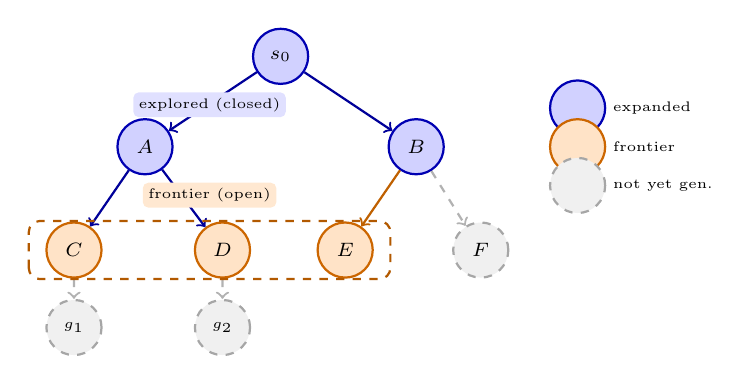
\begin{tikzpicture}[scale=0.82,every node/.style={font=\scriptsize},
  state/.style={circle,draw,thick,minimum size=7mm,inner sep=1pt},
  frontier/.style={circle,draw=orange!80!black,thick,fill=orange!22,minimum size=7mm},
  explored/.style={circle,draw=blue!70!black,thick,fill=blue!18,minimum size=7mm},
  fringe/.style={circle,draw=gray!70,thick,fill=gray!12,minimum size=7mm,dashed}]
\node[explored] (s0) at (0,3) {$s_0$};
\node[explored] (a) at (-2.1,1.6) {$A$};
\node[explored] (b) at (2.1,1.6) {$B$};
\node[frontier] (c) at (-3.2,0) {$C$};
\node[frontier] (d) at (-0.9,0) {$D$};
\node[frontier] (e) at (1.0,0) {$E$};
\node[fringe] (f) at (3.1,0) {$F$};
\node[fringe] (g) at (-3.2,-1.2) {\tiny $g_1$};
\node[fringe] (h) at (-0.9,-1.2) {\tiny $g_2$};
\draw[->,thick,blue!60!black] (s0)--(a);
\draw[->,thick,blue!60!black] (s0)--(b);
\draw[->,thick,blue!60!black] (a)--(c);
\draw[->,thick,blue!60!black] (a)--(d);
\draw[->,thick,orange!75!black] (b)--(e);
\draw[->,thick,gray!60,dashed] (b)--(f);
\draw[->,thick,gray!60,dashed] (c)--(g);
\draw[->,thick,gray!60,dashed] (d)--(h);
% frontier band
\draw[orange!70!black,thick,rounded corners=4pt,dashed] (-3.9,-0.45) rectangle (1.7,0.45);
\node[font=\tiny,fill=orange!18,rounded corners=2pt,inner sep=2pt] at (-1.1,0.85) {frontier (open)};
\node[font=\tiny,fill=blue!12,rounded corners=2pt,inner sep=2pt] at (-1.1,2.25) {explored (closed)};
% legend
\node[explored,font=\tiny] at (4.6,2.2) {$ $}; \node[font=\tiny,anchor=west] at (5.0,2.2) {expanded};
\node[frontier,font=\tiny] at (4.6,1.6) {$ $}; \node[font=\tiny,anchor=west] at (5.0,1.6) {frontier};
\node[fringe,font=\tiny] at (4.6,1.0) {$ $}; \node[font=\tiny,anchor=west] at (5.0,1.0) {not yet gen.};
\end{tikzpicture}
\caption{Search tree vs.\ state space. Blue = explored (already expanded), orange solid = frontier (generated, unexpanded), dashed grey = not yet generated. Graph search would prune a successor already in blue/orange.}
\label{fig:search-tree-frontier}
\end{figure}

General graph search loops: pop a node from \emph{frontier}; test goal; add state to \emph{explored}; expand and insert unseen successors into frontier. The frontier's queueing discipline determines the algorithm.

% ============================================================
\section{Breadth-First and Depth-First Search}
\label{sec:bfs-dfs}
\emph{BFS} uses a FIFO queue (frontier = queue): expand shallowest nodes first, level by level. \emph{DFS} uses a LIFO stack: plunge down one branch before backtracking. Fig.~\ref{fig:bfs-dfs-compare} shows the order in which nodes are expanded on the same tree.

If branching factor is $b$, shallowest goal depth is $d$, and maximum depth is $m$: BFS is \emph{complete} (finds a goal if one exists) and \emph{optimal} when all step costs are equal (first goal found is shallowest). It costs $O(b^d)$ time and $O(b^d)$ memory---memory is the bottleneck. DFS needs only $O(bm)$ memory (the path plus siblings) and $O(b^m)$ time, but is \emph{neither complete} (infinite branches) nor optimal in general; graph-search with cycle checking restores completeness on finite spaces.

\begin{figure}[h]
\centering
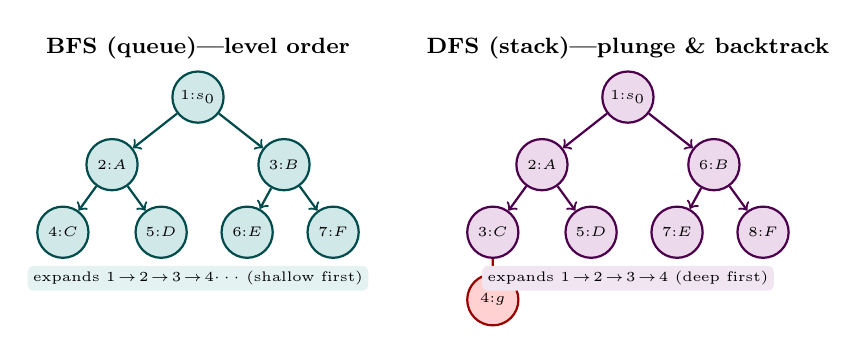
\begin{tikzpicture}[scale=0.78,every node/.style={font=\scriptsize},
  nstyle/.style={circle,draw,thick,minimum size=6.5mm,inner sep=1pt},
  bfs/.style={nstyle,fill=teal!18,draw=teal!60!black},
  dfs/.style={nstyle,fill=violet!15,draw=violet!60!black}]
% BFS tree left
\begin{scope}
\node[font=\footnotesize\bfseries] at (0,3.0) {BFS (queue)---level order};
\node[bfs] (b0) at (0,2.2) {\tiny 1:$s_0$};
\node[bfs] (b1) at (-1.4,1.1) {\tiny 2:$A$};
\node[bfs] (b2) at (1.4,1.1) {\tiny 3:$B$};
\node[bfs] (b3) at (-2.2,0) {\tiny 4:$C$};
\node[bfs] (b4) at (-0.6,0) {\tiny 5:$D$};
\node[bfs] (b5) at (0.8,0) {\tiny 6:$E$};
\node[bfs] (b6) at (2.2,0) {\tiny 7:$F$};
\draw[->,thick,teal!60!black] (b0)--(b1); \draw[->,thick,teal!60!black] (b0)--(b2);
\draw[->,thick,teal!60!black] (b1)--(b3); \draw[->,thick,teal!60!black] (b1)--(b4);
\draw[->,thick,teal!60!black] (b2)--(b5); \draw[->,thick,teal!60!black] (b2)--(b6);
\node[font=\tiny,fill=teal!10,rounded corners=2pt,inner sep=2pt] at (0,-0.75) {expands $1\!\to\!2\!\to\!3\!\to\!4\!\cdots$ (shallow first)};
\end{scope}
% DFS tree right
\begin{scope}[xshift=7.0cm]
\node[font=\footnotesize\bfseries] at (0,3.0) {DFS (stack)---plunge \& backtrack};
\node[dfs] (d0) at (0,2.2) {\tiny 1:$s_0$};
\node[dfs] (d1) at (-1.4,1.1) {\tiny 2:$A$};
\node[dfs] (d2) at (1.4,1.1) {\tiny 6:$B$};
\node[dfs] (d3) at (-2.2,0) {\tiny 3:$C$};
\node[dfs] (d4) at (-0.6,0) {\tiny 5:$D$};
\node[dfs] (d5) at (0.8,0) {\tiny 7:$E$};
\node[dfs] (d6) at (2.2,0) {\tiny 8:$F$};
\node[dfs,fill=red!18,draw=red!60!black] (d7) at (-2.2,-1.1) {\tiny 4:$g$};
\draw[->,thick,violet!60!black] (d0)--(d1); \draw[->,thick,violet!60!black] (d0)--(d2);
\draw[->,thick,violet!60!black] (d1)--(d3); \draw[->,thick,violet!60!black] (d1)--(d4);
\draw[->,thick,violet!60!black] (d2)--(d5); \draw[->,thick,violet!60!black] (d2)--(d6);
\draw[->,thick,red!60!black] (d3)--(d7);
\node[font=\tiny,fill=violet!10,rounded corners=2pt,inner sep=2pt] at (0,-0.75) {expands $1\!\to\!2\!\to\!3\!\to\!4$ (deep first)};
\end{scope}
\end{tikzpicture}
\caption{BFS vs.\ DFS expansion order (numbers) on the same tree. BFS finds shallow goals first; DFS dives to depth $m$ with far less memory. Orange frontier in Fig.~\ref{fig:search-tree-frontier} becomes a queue (BFS) or stack (DFS).}
\label{fig:bfs-dfs-compare}
\end{figure}

\begin{lstlisting}[language=Python,caption={Breadth-first search (graph search, FIFO frontier). Returns path or None.},label={lst:bfs}]
from collections import deque

def bfs(problem):
    """problem: object with initial, is_goal(s), successors(s)->list[s], cost(s,s')."""
    start = problem.initial
    if problem.is_goal(start):
        return [start]
    frontier = deque([[start]])          # queue of paths
    explored = {start}
    while frontier:
        path = frontier.popleft()        # FIFO -> BFS
        s = path[-1]
        for ns in problem.successors(s):
            if ns not in explored:
                if problem.is_goal(ns):
                    return path + [ns]
                explored.add(ns)
                frontier.append(path + [ns])
    return None
\end{lstlisting}

% ============================================================
\section{Uniform-Cost Search and Iterative Deepening}
\label{sec:ucs-ids}
When $c(s,a,s')$ varies, shallowest $\neq$ cheapest. \emph{Uniform-cost search (UCS)} is BFS with costs: frontier is a priority queue ordered by $g(n)$ (path cost from $s_0$). It expands nodes in increasing $g$---exactly Dijkstra's algorithm. UCS is complete and optimal when $c\ge\epsilon>0$, with $O(b^{1+C^*/\epsilon})$ time where $C^*$ is optimal cost.

\emph{Iterative deepening search (IDS)} runs DFS with depth limit $l=0,1,2,\dots$ until a goal is found. Each iteration re-expands upper levels, but the overhead is small: $\sum_{i=0}^{d}b^i / b^d \approx b/(b-1)$. IDS is complete and optimal for uniform costs, with BFS's optimality but DFS's $O(bd)$ memory---the preferred blind method when $b$ is moderate and $d$ unknown. The depth-limited subroutine is just DFS that cuts off at depth $l$.

\begin{lstlisting}[language=Python,caption={Depth-limited DFS and iterative deepening (graph search with depth cap).},label={lst:ids}]
def dls(problem, limit):
    """Depth-limited DFS; returns path or None. Uses stack (LIFO)."""
    frontier = [([problem.initial], 0)]  # (path, depth)
    explored = set()
    while frontier:
        path, d = frontier.pop()         # LIFO -> DFS
        s = path[-1]
        if problem.is_goal(s):
            return path
        if d < limit and s not in explored:
            explored.add(s)
            for ns in reversed(problem.successors(s)):
                if ns not in explored:
                    frontier.append((path + [ns], d + 1))
    return None

def ids(problem, max_depth=50):
    for lim in range(max_depth + 1):
        res = dls(problem, lim)
        if res is not None:
            return res
    return None
\end{lstlisting}

\begin{table}[h]
\centering\small
\begin{tabular}{lcccc}
\toprule
Criterion & BFS & DFS (graph) & UCS & IDS \\
\midrule
Complete & Yes & Yes* & Yes ($c\!\ge\!\epsilon$) & Yes \\
Optimal (uniform/equal cost) & Yes & No & Yes (any $c$) & Yes \\
Time & $O(b^d)$ & $O(b^m)$ & $O(b^{1+C^*/\epsilon})$ & $O(b^d)$ \\
Space & $O(b^d)$ & $O(bm)$ & $O(b^{1+C^*/\epsilon})$ & $O(bd)$ \\
Frontier & FIFO queue & LIFO stack & priority by $g$ & LIFO + depth limit \\
\bottomrule
\end{tabular}
\caption{Blind search at a glance. $b$ = branching, $d$ = goal depth, $m$ = max depth, $C^*$ = optimal cost. {\footnotesize *Graph-DFS complete on finite spaces; tree-DFS can cycle forever.}}
\label{tab:uninformed-compare}
\end{table}

% ============================================================
\section{Chapter Notes}
Blind search was formalised in early AI (Newell \& Simon, 1963; Nilsson, 1971). BFS/DFS are graph traversals from the 19th century (Tr\'emaux, Tarry); UCS is Dijkstra (1959) recast for AI. IDS (Korf, 1985) shows that repetition can buy memory. All strategies here are \emph{uninformed}---they use no estimate of distance to goal; Ch.~3 adds heuristics ($A^*$) to guide the frontier.

% ============================================================
\section{Exercises}
\label{sec:ch02-exercises}
\begin{enumerate}[label=E2.\arabic*, leftmargin=*, itemsep=0.8em]
\item \textbf{Formulation.} Formalise 8-puzzle as $(S,A,\text{Succ},s_0,G,c)$. What is $|S|$ (reachable)? Give $b$ (avg branching) and why Manhattan distance is not part of this chapter's blind search.
\item \textbf{Tree vs.\ graph.} On a grid with 4-neighbour moves, start $(0,0)$, goal $(2,1)$, no obstacles. Draw the search tree to depth 2. How many tree nodes vs.\ distinct states? Which duplicate states does graph search prune at depth 2?
\item \textbf{BFS/DFS/UCS by hand.} Graph: $s_0\!\to\!A(2),B(1); A\!\to\!G(2); B\!\to\!A(1),G(5)$ where $(c)$ is edge cost. Give expansion order and returned path for (a) BFS, (b) DFS (alphabetic successor order), (c) UCS. Which are optimal?
\item \textbf{IDS cost.} Prove IDS expands $N_{\text{IDS}}=\sum_{i=0}^{d}(d+1-i)b^i$ nodes and $N_{\text{BFS}}=\sum_{i=0}^{d}b^i$. Show $N_{\text{IDS}}/N_{\text{BFS}}\to b/(b-1)$ as $d$ grows, and evaluate for $b=10,d=6$.
\item \textbf{Programming.} Implement \texttt{bfs} and \texttt{ids} above on a Romania map (8--10 cities). Compare nodes expanded and max frontier size for Arad$\to$Bucharest. Verify BFS expands $\Theta(b^d)$ nodes while IDS uses $O(bd)$ frontier memory.
\end{enumerate}
% End of Chapter 2
